%!tex root=./thesis.tex

\chapter*{Appendix}
\addcontentsline{toc}{chapter}{Appendix}

\appendix

\section{Accuracy tables}\label{sec:atlas-xid-accuracies}
  
  This section contains tables of accuracy for our method applied to CDFS and
  ELAIS-S1. In \autoref{tab:cdfs-ba} and \autoref{tab:elais-ba} we list the
  balanced accuracies of classifiers on the cross-identification task for CDFS
  and ELAIS-S1 respectively, averaged over each set of training quadrants. In
  \autoref{tab:cdfs-acc} and \autoref{tab:elais-acc} we list the balanced
  accuracies of classifiers on the cross-identification task for CDFS and
  ELAIS-S1 respectively, averaged over each set of training quadrants.

  \begin{table*}
    \caption{Balanced accuracies for different binary classification models trained and tested on SWIRE objects in CDFS.
    The `Labeller' column states what set of training labels
    were used to train the classifier, and the `Classifier' column states what
    classification model was used. `CNN' is a convolutional neural network,
    `LR' is logistic regression and `RF' is random forests. Accuracies are evaluated against the expert
    label set derived from \citet{norris06}. The standard deviation of balanced accuracies evaluated across the four quadrants of
    CDFS (\autoref{fig:quadrants}) is also shown. The `compact' set refers to SWIRE
    objects within $1'$ of a compact radio component, the `resolved' set refers to
    SWIRE objects within $1'$ of a resolved radio component, and `all' is the union of these sets.}
    \label{tab:cdfs-ba}
    \begin{tabular}{ccccc}
    \hline
    Labeller & Classifier & Mean `Compact' accuracy & Mean `Resolved' accuracy & Mean `All' accuracy\\
     &  & (per cent) & (per cent) & (per cent)\\
    \hline
    Norris & LR & $91.5 \pm 1.0$ & $93.2 \pm 1.0$ & $93.0 \pm 1.2$\\
    Norris & CNN & $92.6 \pm 0.7$ & $91.2 \pm 0.5$ & $92.0 \pm 0.6$\\
    Norris & RF & $96.7 \pm 1.5$ & $91.0 \pm 4.5$ & $96.0 \pm 2.5$\\
    RGZ & LR & $89.5 \pm 0.8$ & $90.5 \pm 1.7$ & $90.2 \pm 0.8$\\
    RGZ & CNN & $89.4 \pm 0.6$ & $89.6 \pm 1.3$ & $89.4 \pm 0.5$\\
    RGZ & RF & $94.5 \pm 0.2$ & $95.8 \pm 0.4$ & $94.7 \pm 0.3$\\
    \hline
    \end{tabular}
  \end{table*}

  \begin{table*}
    \caption{Balanced accuracies for different binary classification models trained on SWIRE objects
    in CDFS and tested on SWIRE objects in ELAIS-S1. Columns and abbreviations are as in \autoref{tab:cdfs-ba}. Accuracies are evaluated against the expert
    label set derived from \citet{middelberg08}. The standard deviations of balanced accuracies of models trained on the four subsets of
    CDFS (\autoref{fig:quadrants}) are also shown.}
    \label{tab:elais-ba}
    \begin{tabular}{ccccc}
      \hline
      Labeller & Classifier & Mean `Compact' accuracy & Mean `Resolved' accuracy & Mean `All' accuracy\\
        &  & (per cent) & (per cent) & (per cent)\\
      \hline
      Norris & LR & $94.6 \pm 0.4$ & $93.3 \pm 2.0$ & $95.3 \pm 0.1$\\
       & CNN & $94.8 \pm 0.2$ & $92.8 \pm 0.5$ & $94.4 \pm 0.2$\\
       & RF & $85.9 \pm 3.8$ & $70.0 \pm 2.8$ & $86.6 \pm 3.2$\\
      RGZ & LR & $91.8 \pm 0.3$ & $91.9 \pm 0.5$ & $92.0 \pm 0.2$\\
       & CNN & $90.1 \pm 0.3$ & $91.1 \pm 0.9$ & $90.2 \pm 0.3$\\
       & RF & $95.1 \pm 0.1$ & $95.2 \pm 0.0$ & $95.2 \pm 0.3$\\
      \hline
    \end{tabular}
  \end{table*}

  \begin{table*}
    \caption{Cross-identification accuracies for different classification
    models on CDFS. The `Labeller' column states what set of training labels
    were used to train the method, and the `Classifier' column states what
    classification model was used. `CNN' is a convolutional neural network,
    `LR' is logistic regression, `RF' is random forests, and `Labels' is the
    accuracy of the label set itself. `Perfect' indicates that the true labels
    of the test set were used and hence represents an upper bound on
    cross-identification accuracy with our method. `NN' is a
    nearest-neighbours approach. Accuracies are evaluated against the expert
    label set, so `Norris' labels are 100 per cent accurate by definition. The
    standard deviation of accuracies evaluated across the four quadrants of
    CDFS (\autoref{fig:quadrants}) is also shown.}
    \label{tab:cdfs-acc}
    \begin{tabular}{ccccc}
      \hline
      Labeller & Classifier & Mean `Compact' accuracy & Mean `Resolved' accuracy & Mean `All' accuracy\\
       &  & (per cent) & (per cent) & (per cent)\\
      \hline
      --- & NN & $97.2 \pm 1.7$ & $75.7 \pm 7.9$ & $93.4 \pm 0.8$\\
      --- & Random & $97.9 \pm 2.2$ & $22.3 \pm 9.2$ & $83.2 \pm 4.7$\\
      Norris & Labels & $100.0 \pm 0.0$ & $100.0 \pm 0.0$ & $100.0 \pm 0.0$\\
             & Perfect & $97.9 \pm 2.2$ & $99.0 \pm 1.8$ & $98.1 \pm 1.7$\\
             & LR & $97.3 \pm 0.5$ & $76.0 \pm 3.2$ & $93.7 \pm 1.8$\\
             & CNN & $96.6 \pm 0.9$ & $74.3 \pm 12.3$ & $93.5 \pm 0.5$\\
             & RF & $96.1 \pm 1.4$ & $75.8 \pm 6.7$ & $93.8 \pm 2.0$\\
      RGZ & Labels & $53.1 \pm 8.5$ & $56.7 \pm 5.9$ & $54.4 \pm 5.9$\\
          & LR & $97.3 \pm 1.9$ & $74.5 \pm 5.1$ & $93.6 \pm 1.7$\\
          & CNN & $85.4 \pm 2.6$ & $68.1 \pm 9.2$ & $92.4 \pm 1.1$\\
          & RF & $97.5 \pm 0.9$ & $74.3 \pm 7.9$ & $93.7 \pm 1.5$\\
      \hline
    \end{tabular}
  \end{table*}

  \begin{table*}
    \caption{Cross-identification accuracies for different classification
    models on ELAIS-S1. Columns and abbreviations are as in
    \autoref{tab:cdfs-acc}. Accuracies are evaluated against the expert label
    set derived from \citet{middelberg08} cross-identifications. The standard
    deviation of accuracies evaluated across models trained on the four
    quadrants of CDFS (\autoref{fig:quadrants}) is also shown.}
    \label{tab:elais-acc}
    \begin{tabular}{ccccc}
      \hline
      Labeller & Classifier & Mean `Compact' accuracy & Mean `Resolved' accuracy & Mean `All' accuracy\\
       &  & (per cent) & (per cent) & (per cent)\\
      \hline
      --- & NN & $95.5 \pm 0.0$ & $92.8 \pm 0.0$ & $95.5 \pm 0.0$\\
      --- & Random & $61.9 \pm 1.1$ & $26.6 \pm 2.1$ & $61.9 \pm 1.1$\\
      Middelberg & Perfect & $99.6 \pm 0.0$ & $99.8 \pm 0.0$ & $99.6 \pm 0.0$\\
      Norris & LR & $89.0 \pm 1.1$ & $89.7 \pm 1.8$ & $94.4 \pm 0.9$\\
             & CNN & $89.7 \pm 0.3$ & $89.4 \pm 1.4$ & $94.3 \pm 0.7$\\
             & RF & $83.8 \pm 5.6$ & $82.3 \pm 4.1$ & $90.6 \pm 2.1$\\
      RGZ & LR & $90.5 \pm 1.0$ & $92.7 \pm 0.2$ & $95.9 \pm 0.1$\\
          & CNN & $84.6 \pm 0.6$ & $84.6 \pm 0.6$ & $91.8 \pm 0.3$\\
          & RF & $91.3 \pm 1.0$ & $90.3 \pm 2.4$ & $94.7 \pm 1.2$\\
      \hline
    \end{tabular}
  \end{table*}

\section{SWIRE object scores}\label{sec:atlas-xid-scores}
  
  This section contains scores predicted by our binary classifiers for each
  SWIRE object within $1'$ of a radio component in CDFS and ELAIS-S1. Scores
  for SWIRE~CDFS objects are shown in \autoref{tab:cdfs-scores} and scores for
  SWIRE~ELAIS-S1 are shown in \autoref{tab:elais-scores}. For CDFS, the score
  for an object in a quadrant is predicted by binary classifiers trained on
  all other quadrants. For ELAIS-S1, we show the scores predicted by binary
  classifiers trained on each CDFS quadrant. Note that these scores have
  \emph{not} been weighted by Gaussians.

  The columns of the score tables are defined as follows:
  \begin{itemize}
    \item \emph{SWIRE} --- SWIRE designation for candidate host galaxy.
    \item \emph{RA} --- Right ascension (J2000).
    \item \emph{Dec} --- Declination (J2000).
    \item \emph{Expert host} --- Whether the candidate host galaxy is a host galaxy according to \citet{norris06} or \citet{middelberg08} cross-identifications of CDFS and ELAIS-S1 respectively.
    \item \emph{RGZ host} --- Whether the candidate host galaxy is a host galaxy according to Radio Galaxy Zoo cross-identifications (Wong et al. in prep). This is always "no" for ELAIS-S1 objects.
    \item \emph{$C$($L$ / $D$)} --- Score assigned by binary classifier $C$ trained on label set $L$ of $D$ candidate host galaxies. $C$ may be `CNN', `LR' or `RF' for CNN, logistic regression or random forests respectively. $L$ may be `Norris' or `RGZ' for expert and Radio Galaxy Zoo labels respectively. $D$ may be `All', `Compact' or `Resolved' for each respective subset defined in \autoref{sec:atlas-xid-experimental-setup}.
  \end{itemize}

  \begin{table}
    \caption{Scores output by our trained classifiers for SWIRE~CDFS candidate host galaxies. Columns are defined in \autoref{sec:atlas-xid-scores}. Full table electronic.}
    \label{tab:cdfs-scores}
    \begin{tabular}{ccccccccccccccccccccccc}
      \hline
SWIRE & RA & Dec & Expert host & RGZ host & CNN(Norris / All) & CNN(Norris / Compact) & CNN(Norris / Resolved) & CNN(RGZ / All) & CNN(RGZ / Compact) & CNN(RGZ / Resolved) & LR(Norris / All) & LR(Norris / Compact) & LR(Norris / Resolved) & LR(RGZ / All) & LR(RGZ / Compact) & LR(RGZ / Resolved) & RF(Norris / All) & RF(Norris / Compact) & RF(Norris / Resolved) & RF(RGZ / All) & RF(RGZ / Compact) & RF(RGZ / Resolved) \\
      \hline
J032603.15-284708.5 & 51.5132 & -28.7857 & yes & no & 0.5838 & 0.4697 & 0.4848 & 0.3754 & 0.3881 & 0.3404 & 0.2489 & 0.0009 & 0.1557 & 0.2939 & 0.0007 & 0.1174 & 0.8922 & 0.8018 & 0.8732 & 0.7167 & 0.6599 & 0.7801 \\
J032603.39-284010.1 & 51.5142 & -28.6695 & no & no & 0.0373 & 0.5814 & 0.4878 & 0.7896 & 0.7616 & 0.4668 & 0.0183 & 0.1646 & 0.1480 & 0.7637 & 0.7065 & 0.6070 & 0.0000 & 0.0000 & 0.0000 & 0.1629 & 0.0519 & 0.1275 \\
J032603.44-284210.1 & 51.5144 & -28.7028 & no & no & 0.0232 & 0.4891 & 0.5101 & 0.4319 & 0.4298 & 0.3474 & 0.0155 & 0.0164 & 0.0815 & 0.3714 & 0.5626 & 0.2488 & 0.0000 & 0.0734 & 0.0000 & 0.1315 & 0.2116 & 0.4150 \\
J032603.44-284222.2 & 51.5143 & -28.7062 & no & no & 0.0006 & 0.4164 & 0.5216 & 0.0400 & 0.0444 & 0.0276 & 0.0005 & 0.0006 & 0.0175 & 0.0460 & 0.0810 & 0.0299 & 0.2656 & 0.1418 & 0.0000 & 0.7631 & 0.8166 & 0.5378 \\
J032603.45-284748.4 & 51.5144 & -28.7968 & no & no & 0.0014 & 0.4914 & 0.4865 & 0.1904 & 0.1895 & 0.1467 & 0.0013 & 0.0037 & 0.0160 & 0.1792 & 0.0663 & 0.1821 & 0.0000 & 0.0000 & 0.0000 & 0.0255 & 0.0000 & 0.0000 \\
J032603.50-284637.0 & 51.5146 & -28.7770 & no & no & 0.0074 & 0.4144 & 0.5382 & 0.1418 & 0.1515 & 0.1166 & 0.0047 & 0.0010 & 0.0337 & 0.1284 & 0.2198 & 0.0694 & 0.0720 & 0.0000 & 0.0000 & 0.6240 & 0.6681 & 0.6704 \\
J032603.60-284627.4 & 51.5150 & -28.7743 & no & no & 0.0012 & 0.4578 & 0.5165 & 0.0850 & 0.0904 & 0.0484 & 0.0008 & 0.0006 & 0.0374 & 0.1053 & 0.1424 & 0.0807 & 0.1231 & 0.0876 & 0.0000 & 0.8517 & 0.7532 & 0.7019 \\
J032603.63-283840.5 & 51.5151 & -28.6446 & no & no & 0.0021 & 0.4153 & 0.5577 & 0.1678 & 0.1746 & 0.1323 & 0.0021 & 0.0073 & 0.0386 & 0.1482 & 0.0403 & 0.1210 & 0.0000 & 0.0532 & 0.0000 & 0.0000 & 0.0302 & 0.0000 \\
J032603.66-283822.8 & 51.5153 & -28.6397 & no & no & 0.0001 & 0.4752 & 0.5009 & 0.0864 & 0.0861 & 0.0613 & 0.0001 & 0.0004 & 0.0038 & 0.0854 & 0.0447 & 0.0514 & 0.0000 & 0.0000 & 0.0000 & 0.0000 & 0.0000 & 0.0000 \\
J032603.75-284014.1 & 51.5156 & -28.6706 & no & no & 0.0547 & 0.3408 & 0.5388 & 0.4889 & 0.5242 & 0.7301 & 0.0542 & 0.2712 & 0.2318 & 0.5026 & 0.5631 & 0.5032 & 0.0595 & 0.0545 & 0.0000 & 0.4289 & 0.0789 & 0.1420 \\
      \hline
    \end{tabular}
  \end{table}

  \begin{table}
    \caption{Scores output by our trained classifiers for SWIRE~ELAIS-S1 candidate host galaxies. Columns are defined in \autoref{sec:atlas-xid-scores}. Full table electronic.}
    \label{tab:elais-scores}
    \begin{tabular}{ccccccccccccccccccccccc}
      \hline
SWIRE & RA & Dec & Expert host & RGZ host & CNN(Norris / All) & CNN(Norris / Compact) & CNN(Norris / Resolved) & CNN(RGZ / All) & CNN(RGZ / Compact) & CNN(RGZ / Resolved) & LR(Norris / All) & LR(Norris / Compact) & LR(Norris / Resolved) & LR(RGZ / All) & LR(RGZ / Compact) & LR(RGZ / Resolved) & RF(Norris / All) & RF(Norris / Compact) & RF(Norris / Resolved) & RF(RGZ / All) & RF(RGZ / Compact) & RF(RGZ / Resolved) \\
      \hline
J002925.73-440256.2 & 7.3572 & -44.0490 & yes & no & 0.9537 & 0.8638 & 0.5552 & 0.9195 & 0.9037 & 0.9371 & 0.9722 & 0.9955 & 0.8769 & 0.9933 & 0.9934 & 0.9658 & 0.8824 & 0.9664 & 0.7950 & 0.8078 & 0.9227 & 0.7677 \\
J002926.14-440249.0 & 7.3590 & -44.0470 & no & no & 0.7361 & 0.8752 & 0.5640 & 0.7740 & 0.7474 & 0.7952 & 0.4669 & 0.0111 & 0.4249 & 0.3926 & 0.2220 & 0.5947 & 0.2077 & 0.0000 & 0.1613 & 0.1876 & 0.0852 & 0.4546 \\
J002926.52-440247.0 & 7.3605 & -44.0464 & no & no & 0.3390 & 0.8338 & 0.5556 & 0.7275 & 0.6894 & 0.7197 & 0.2264 & 0.0254 & 0.2389 & 0.6275 & 0.3033 & 0.6812 & 0.1347 & 0.0857 & 0.0399 & 0.3582 & 0.4854 & 0.5347 \\
J002926.63-440301.1 & 7.3610 & -44.0503 & no & no & 0.2108 & 0.8251 & 0.5623 & 0.3434 & 0.3306 & 0.3292 & 0.0603 & 0.0007 & 0.0734 & 0.0688 & 0.0141 & 0.1581 & 0.0917 & 0.0000 & 0.0399 & 0.2846 & 0.1245 & 0.2833 \\
J002927.13-440232.6 & 7.3631 & -44.0424 & no & no & 0.0339 & 0.8479 & 0.5669 & 0.5853 & 0.5148 & 0.5159 & 0.0248 & 0.0334 & 0.0301 & 0.5735 & 0.5065 & 0.5265 & 0.1977 & 0.1507 & 0.0000 & 0.3334 & 0.6593 & 0.3995 \\
J002927.28-440245.3 & 7.3637 & -44.0459 & no & no & 0.0406 & 0.8345 & 0.5540 & 0.2702 & 0.2340 & 0.2133 & 0.0173 & 0.0016 & 0.0359 & 0.1056 & 0.0492 & 0.1456 & 0.0000 & 0.0000 & 0.0000 & 0.0000 & 0.0000 & 0.0287 \\
J002927.44-440238.5 & 7.3644 & -44.0440 & no & no & 0.0116 & 0.8267 & 0.5746 & 0.2228 & 0.2182 & 0.2028 & 0.0064 & 0.0049 & 0.0187 & 0.1981 & 0.1534 & 0.1493 & 0.0000 & 0.0000 & 0.0000 & 0.1565 & 0.1634 & 0.1284 \\
J002928.08-440230.3 & 7.3670 & -44.0418 & no & no & 0.0024 & 0.8626 & 0.5791 & 0.2297 & 0.1963 & 0.1549 & 0.0020 & 0.0005 & 0.0239 & 0.1337 & 0.1001 & 0.1310 & 0.0000 & 0.0000 & 0.0358 & 0.0000 & 0.0000 & 0.0190 \\
J002928.11-440312.7 & 7.3671 & -44.0535 & no & no & 0.0011 & 0.8159 & 0.5514 & 0.0377 & 0.0384 & 0.0271 & 0.0008 & 0.0013 & 0.0119 & 0.0280 & 0.0361 & 0.0205 & 0.1171 & 0.0000 & 0.0000 & 0.0873 & 0.0383 & 0.0000 \\
J002928.80-440306.8 & 7.3700 & -44.0519 & no & no & 0.0003 & 0.8405 & 0.5668 & 0.0236 & 0.0226 & 0.0136 & 0.0004 & 0.0014 & 0.0095 & 0.0339 & 0.0408 & 0.0136 & 0.0000 & 0.0000 & 0.0000 & 0.1114 & 0.1480 & 0.1584 \\
      \hline
    \end{tabular}
  \end{table}

\section{ATLAS component cross-identifications}\label{sec:atlas-xids}
  
  This section contains cross-identifications predicted by our method for each
  ATLAS radio component in CDFS and ELAIS-S1. Cross-identifications for
  ATLAS~CDFS components are shown in \autoref{tab:cdfs-xids} and
  cross-identifications for ATLAS~ELAIS-S1 are shown in
  \autoref{tab:elais-xids}. For CDFS, the cross-identification for a component
  in a quadrant is predicted using our method with binary classifiers trained
  on all other quadrants. For ELAIS-S1, we show the cross-identifications
  predicted by our method using binary classifiers trained on each CDFS
  quadrant. For CDFS, we also show the Radio Galaxy Zoo consensus, which is a
  proxy for the difficulty of cross-identifying a component (Wong et al. in
  prep).

  The columns of the cross-identification tables are defined as follows:
  \begin{itemize}
    \item \emph{ATLAS} --- ATLAS designation for radio component.
    \item \emph{RA} --- Right ascension of radio component (J2000).
    \item \emph{Dec} --- Declination of radio component (J2000).
    \item \emph{CID} --- Radio Galaxy Zoo component ID.
    \item \emph{Zooniverse ID} --- Radio Galaxy Zoo Zooniverse ID.
    \item \emph{Norris/Middelberg} --- Designation of SWIRE cross-identification from \citet{norris06} or \citet{middelberg08} for CDFS and ELAIS-S1 respectively.
    \item \emph{Norris/Middelberg RA} --- Right ascension of SWIRE cross-identification from \citet{norris06} or \citet{middelberg08} for CDFS and ELAIS-S1 respectively.
    \item \emph{Norris/Middelberg Dec} --- Right ascension of SWIRE cross-identification from \citet{norris06} or \citet{middelberg08} for CDFS and ELAIS-S1 respectively.
    \item \emph{RGZ} --- Designation of SWIRE cross-identification from Radio Galaxy Zoo (Wong et al. in prep).
    \item \emph{RGZ RA} --- Right ascension of SWIRE cross-identification from Radio Galaxy Zoo (Wong et al. in prep).
    \item \emph{RGZ Dec} --- Right ascension of SWIRE cross-identification from Radio Galaxy Zoo (Wong et al. in prep).
    \item \emph{RGZ radio consensus} --- Percentage agreement of Radio Galaxy Zoo volunteers on the radio component configuration.
    \item \emph{RGZ IR consensus} --- Percentage agreement of Radio Galaxy Zoo volunteers on the host galaxy of this radio component.
    \item \emph{$C$($L$ / $D$)} --- Designation of SWIRE cross-identification made by our method using classification model $C$ trained on label set $L$ of $D$ candidate host galaxies. $C$ may be `CNN', `LR' or `RF' for CNN, logistic regression or random forests respectively. $L$ may be `Norris' or `RGZ' for expert and Radio Galaxy Zoo labels respectively. $D$ may be `All', `Compact' or `Resolved' for each respective subset defined in \autoref{sec:atlas-xid-experimental-setup}.
    \item \emph{$C$($L$ / $D$) RA} --- Right ascension (J2000) of SWIRE cross-identification made by our method using classification model $C$ trained on label set $L$ of $D$ candidate host galaxies. $C$, $L$ and $D$ are defined as for designation.
    \item \emph{$C$($L$ / $D$) Dec} --- Declination (J2000) of SWIRE cross-identification made by our method using classification model $C$ trained on label set $L$ of $D$ candidate host galaxies. $C$, $L$ and $D$ are defined as for designation.
  \end{itemize}

  \begin{table*}
    \caption{Cross-identifications for ATLAS~CDFS components. Columns are defined in \autoref{sec:atlas-xids}. Full table electronic.}
    \label{tab:cdfs-xids}
    \begin{tabular}{ccccccccccccccccccccccccccccccccccccccccccccccccc}
      \hline
ATLAS & RA & Dec & CID & Zooniverse ID & Norris & Norris RA & Norris Dec & RGZ & RGZ RA & RGZ Dec & RGZ radio consensus & RGZ IR consensus & CNN(Norris / Compact) & CNN(Norris / Compact) RA & CNN(Norris / Compact) Dec & CNN(Norris / Resolved) & CNN(Norris / Resolved) RA & CNN(Norris / Resolved) Dec & CNN(RGZ / Compact) & CNN(RGZ / Compact) RA & CNN(RGZ / Compact) Dec & CNN(RGZ / Resolved) & CNN(RGZ / Resolved) RA & CNN(RGZ / Resolved) Dec & LR(Norris / Compact) & LR(Norris / Compact) RA & LR(Norris / Compact) Dec & LR(Norris / Resolved) & LR(Norris / Resolved) RA & LR(Norris / Resolved) Dec & LR(RGZ / Compact) & LR(RGZ / Compact) RA & LR(RGZ / Compact) Dec & LR(RGZ / Resolved) & LR(RGZ / Resolved) RA & LR(RGZ / Resolved) Dec & RF(Norris / Compact) & RF(Norris / Compact) RA & RF(Norris / Compact) Dec & RF(Norris / Resolved) & RF(Norris / Resolved) RA & RF(Norris / Resolved) Dec & RF(RGZ / Compact) & RF(RGZ / Compact) RA & RF(RGZ / Compact) Dec & RF(RGZ / Resolved) & RF(RGZ / Resolved) RA & RF(RGZ / Resolved) Dec \\
      \hline
J032602.82-284708.1C & 51.5117 & -28.7856 & CI0412 & ARG0003rb2 & J032603.15-284708.5 & 51.5132 & -28.7857 &  &  &  & 0.4516 & 0.3214 & J032602.36-284711.5 & 51.5098 & -28.7865 & J032602.36-284711.5 & 51.5098 & -28.7865 & J032602.36-284711.5 & 51.5098 & -28.7865 & J032602.36-284711.5 & 51.5098 & -28.7865 & J032604.58-284650.9 & 51.5191 & -28.7808 & J032602.08-284713.1 & 51.5087 & -28.787 & J032602.36-284711.5 & 51.5098 & -28.7865 & J032602.36-284711.5 & 51.5098 & -28.7865 & J032603.15-284708.5 & 51.5132 & -28.7857 & J032602.36-284711.5 & 51.5098 & -28.7865 & J032602.36-284711.5 & 51.5098 & -28.7865 & J032602.36-284711.5 & 51.5098 & -28.7865 \\
J032615.49-284629.4C & 51.5646 & -28.7749 & CI0614 & ARG0003rfr & J032615.41-284630.7 & 51.5642 & -28.7752 & J032615.41-284630.7 & 51.5642 & -28.7752 & 0.2941 & 0.8000 & J032615.41-284630.7 & 51.5642 & -28.7752 & J032615.41-284630.7 & 51.5642 & -28.7752 & J032615.41-284630.7 & 51.5642 & -28.7752 & J032615.41-284630.7 & 51.5642 & -28.7752 & J032615.41-284630.7 & 51.5642 & -28.7752 & J032615.41-284630.7 & 51.5642 & -28.7752 & J032615.41-284630.7 & 51.5642 & -28.7752 & J032615.41-284630.7 & 51.5642 & -28.7752 & J032615.41-284630.7 & 51.5642 & -28.7752 & J032615.41-284630.7 & 51.5642 & -28.7752 & J032615.41-284630.7 & 51.5642 & -28.7752 & J032615.41-284630.7 & 51.5642 & -28.7752 \\
J032615.55-280559.8C & 51.5648 & -28.1000 & CI0320 & ARG0003r8s & J032615.52-280559.8 & 51.5647 & -28.1000 & J032615.52-280559.8 & 51.5647 & -28.1000 & 0.5625 & 0.8333 & J032615.52-280559.8 & 51.5647 & -28.1000 & J032615.52-280559.8 & 51.5647 & -28.1000 & J032615.52-280559.8 & 51.5647 & -28.1000 & J032615.52-280559.8 & 51.5647 & -28.1000 & J032615.52-280559.8 & 51.5647 & -28.1000 & J032615.52-280559.8 & 51.5647 & -28.1000 & J032615.52-280559.8 & 51.5647 & -28.1000 & J032615.52-280559.8 & 51.5647 & -28.1000 & J032615.52-280559.8 & 51.5647 & -28.1000 & J032615.52-280559.8 & 51.5647 & -28.1000 & J032615.52-280559.8 & 51.5647 & -28.1000 & J032615.52-280559.8 & 51.5647 & -28.1000 \\
J032617.35-280710.2C & 51.5723 & -28.1195 & CI0059C1 & ARG0003r2j & J032617.89-280707.2 & 51.5746 & -28.1187 & J032617.89-280707.2 & 51.5746 & -28.1187 & 0.4146 & 1.0000 & J032617.89-280707.2 & 51.5746 & -28.1187 & J032617.89-280707.2 & 51.5746 & -28.1187 & J032617.89-280707.2 & 51.5746 & -28.1187 & J032617.89-280707.2 & 51.5746 & -28.1187 & J032615.86-280628.8 & 51.5661 & -28.1080 & J032615.16-280742.2 & 51.5632 & -28.1284 & J032615.86-280628.8 & 51.5661 & -28.1080 & J032618.84-280722.6 & 51.5785 & -28.1230 & J032617.89-280707.2 & 51.5746 & -28.1187 & J032617.89-280707.2 & 51.5746 & -28.1187 & J032617.89-280707.2 & 51.5746 & -28.1187 & J032617.89-280707.2 & 51.5746 & -28.1187 \\
J032625.13-280909.8C & 51.6047 & -28.1527 & CI0409 & ARG0003raz & J032625.19-280910.1 & 51.6050 & -28.1528 & J032625.19-280910.1 & 51.6050 & -28.1528 & 0.3158 & 0.6667 & J032625.19-280910.1 & 51.6050 & -28.1528 & J032625.19-280910.1 & 51.6050 & -28.1528 & J032624.50-280905.9 & 51.6021 & -28.1517 & J032625.19-280910.1 & 51.6050 & -28.1528 & J032625.19-280910.1 & 51.6050 & -28.1528 & J032625.19-280910.1 & 51.6050 & -28.1528 & J032625.19-280910.1 & 51.6050 & -28.1528 & J032625.19-280910.1 & 51.6050 & -28.1528 & J032625.19-280910.1 & 51.6050 & -28.1528 & J032625.19-280910.1 & 51.6050 & -28.1528 & J032625.19-280910.1 & 51.6050 & -28.1528 & J032625.19-280910.1 & 51.6050 & -28.1528 \\
J032629.10-280650.1C & 51.6213 & -28.1139 & CI0963 & ARG0003ro4 & J032629.13-280650.7 & 51.6214 & -28.1141 & J032626.74-280636.7 & 51.6114 & -28.1102 & 0.3333 & 1.0000 & J032629.13-280650.7 & 51.6214 & -28.1141 & J032629.13-280650.7 & 51.6214 & -28.1141 & J032629.13-280650.7 & 51.6214 & -28.1141 & J032629.13-280650.7 & 51.6214 & -28.1141 & J032629.13-280650.7 & 51.6214 & -28.1141 & J032629.13-280650.7 & 51.6214 & -28.1141 & J032629.13-280650.7 & 51.6214 & -28.1141 & J032629.13-280650.7 & 51.6214 & -28.1141 & J032629.13-280650.7 & 51.6214 & -28.1141 & J032629.13-280650.7 & 51.6214 & -28.1141 & J032629.13-280650.7 & 51.6214 & -28.1141 & J032629.13-280650.7 & 51.6214 & -28.1141 \\
J032629.61-284052.7C & 51.6234 & -28.6813 & CI0304 & ARG0003r8e & J032629.54-284055.8 & 51.6231 & -28.6822 & J032629.54-284055.8 & 51.6231 & -28.6822 & 0.2676 & 1.0000 & J032629.54-284051.9 & 51.6231 & -28.6811 & J032629.54-284051.9 & 51.6231 & -28.6811 & J032629.54-284051.9 & 51.6231 & -28.6811 & J032629.54-284051.9 & 51.6231 & -28.6811 & J032629.54-284051.9 & 51.6231 & -28.6811 & J032629.54-284051.9 & 51.6231 & -28.6811 & J032629.54-284051.9 & 51.6231 & -28.6811 & J032629.54-284051.9 & 51.6231 & -28.6811 & J032629.54-284051.9 & 51.6231 & -28.6811 & J032629.54-284051.9 & 51.6231 & -28.6811 & J032629.54-284051.9 & 51.6231 & -28.6811 & J032629.54-284051.9 & 51.6231 & -28.6811 \\
J032629.92-284753.5C & 51.6247 & -28.7982 & CI0120 & ARG0003r3w & J032629.81-284754.4 & 51.6242 & -28.7985 & J032629.81-284754.4 & 51.6242 & -28.7985 & 1.0000 & 0.8571 & J032629.81-284754.4 & 51.6242 & -28.7985 & J032629.81-284754.4 & 51.6242 & -28.7985 & J032629.81-284754.4 & 51.6242 & -28.7985 & J032629.81-284754.4 & 51.6242 & -28.7985 & J032629.81-284754.4 & 51.6242 & -28.7985 & J032629.81-284754.4 & 51.6242 & -28.7985 & J032629.81-284754.4 & 51.6242 & -28.7985 & J032629.81-284754.4 & 51.6242 & -28.7985 & J032630.12-284751.2 & 51.6255 & -28.7976 & J032629.81-284754.4 & 51.6242 & -28.7985 & J032629.81-284754.4 & 51.6242 & -28.7985 & J032629.81-284754.4 & 51.6242 & -28.7985 \\
J032630.66-283657.3C & 51.6278 & -28.6159 & CI0172C1 & ARG0003r55 & J032630.64-283658.0 & 51.6277 & -28.6161 & J032628.56-283744.8 & 51.619 & -28.6291 & 0.3611 & 0.7308 & J032630.64-283658.0 & 51.6277 & -28.6161 & J032630.64-283658.0 & 51.6277 & -28.6161 & J032630.64-283658.0 & 51.6277 & -28.6161 & J032630.64-283658.0 & 51.6277 & -28.6161 & J032630.64-283658.0 & 51.6277 & -28.6161 & J032630.64-283658.0 & 51.6277 & -28.6161 & J032630.64-283658.0 & 51.6277 & -28.6161 & J032630.64-283658.0 & 51.6277 & -28.6161 & J032630.64-283658.0 & 51.6277 & -28.6161 & J032630.64-283658.0 & 51.6277 & -28.6161 & J032630.64-283658.0 & 51.6277 & -28.6161 & J032630.64-283658.0 & 51.6277 & -28.6161 \\
J032634.59-282022.8C & 51.6441 & -28.3397 & CI0757 & ARG0003rj2 & J032634.58-282022.8 & 51.6441 & -28.3397 & J032631.96-281941.0 & 51.6332 & -28.3281 & 0.5781 & 0.5405 & J032634.58-282022.8 & 51.6441 & -28.3397 & J032634.58-282022.8 & 51.6441 & -28.3397 & J032634.58-282022.8 & 51.6441 & -28.3397 & J032634.58-282022.8 & 51.6441 & -28.3397 & J032634.58-282022.8 & 51.6441 & -28.3397 & J032634.58-282022.8 & 51.6441 & -28.3397 & J032634.58-282022.8 & 51.6441 & -28.3397 & J032634.58-282022.8 & 51.6441 & -28.3397 & J032634.58-282022.8 & 51.6441 & -28.3397 & J032634.58-282022.8 & 51.6441 & -28.3397 & J032634.58-282022.8 & 51.6441 & -28.3397 & J032634.58-282022.8 & 51.6441 & -28.3397 \\
      \hline
    \end{tabular}
  \end{table*}

  \begin{table*}
    \caption{Cross-identifications for ATLAS~ELAIS-S1 components. Columns are defined in \autoref{sec:atlas-xids}. Full table electronic.}
    \label{tab:elais-xids}
    \begin{tabular}{ccccccccccccccccccccccccccccccccccccccccccccccccccccccccccccccccccc}
      \hline
ATLAS & RA & Dec & CID & Zooniverse ID & Middelberg & Middelberg RA & Middelberg Dec & RGZ & RGZ RA & RGZ Dec & RGZ radio consensus & RGZ IR consensus & CNN(Norris / All) & CNN(Norris / All) RA & CNN(Norris / All) Dec & CNN(Norris / Compact) & CNN(Norris / Compact) RA & CNN(Norris / Compact) Dec & CNN(Norris / Resolved) & CNN(Norris / Resolved) RA & CNN(Norris / Resolved) Dec & CNN(RGZ / All) & CNN(RGZ / All) RA & CNN(RGZ / All) Dec & CNN(RGZ / Compact) & CNN(RGZ / Compact) RA & CNN(RGZ / Compact) Dec & CNN(RGZ / Resolved) & CNN(RGZ / Resolved) RA & CNN(RGZ / Resolved) Dec & LR(Norris / All) & LR(Norris / All) RA & LR(Norris / All) Dec & LR(Norris / Compact) & LR(Norris / Compact) RA & LR(Norris / Compact) Dec & LR(Norris / Resolved) & LR(Norris / Resolved) RA & LR(Norris / Resolved) Dec & LR(RGZ / All) & LR(RGZ / All) RA & LR(RGZ / All) Dec & LR(RGZ / Compact) & LR(RGZ / Compact) RA & LR(RGZ / Compact) Dec & LR(RGZ / Resolved) & LR(RGZ / Resolved) RA & LR(RGZ / Resolved) Dec & RF(Norris / All) & RF(Norris / All) RA & RF(Norris / All) Dec & RF(Norris / Compact) & RF(Norris / Compact) RA & RF(Norris / Compact) Dec & RF(Norris / Resolved) & RF(Norris / Resolved) RA & RF(Norris / Resolved) Dec & RF(RGZ / All) & RF(RGZ / All) RA & RF(RGZ / All) Dec & RF(RGZ / Compact) & RF(RGZ / Compact) RA & RF(RGZ / Compact) Dec & RF(RGZ / Resolved) & RF(RGZ / Resolved) RA & RF(RGZ / Resolved) Dec \\
      \hline
J002925.68-440256.8 & 7.3570 & -44.0491 & C0375 &  & J002925.73-440256.2 & 7.3572 & -44.0490 &  &  &  &  &  & J002925.73-440256.2 & 7.3572 & -44.049 & J002925.73-440256.2 & 7.3572 & -44.0490 & J002925.73-440256.2 & 7.3572 & -44.0490 & J002925.73-440256.2 & 7.3572 & -44.0490 & J002925.73-440256.2 & 7.3572 & -44.0490 & J002925.73-440256.2 & 7.3572 & -44.0490 & J002925.73-440256.2 & 7.3572 & -44.0490 & J002925.73-440256.2 & 7.3572 & -44.0490 & J002925.73-440256.2 & 7.3572 & -44.0490 & J002925.73-440256.2 & 7.3572 & -44.0490 & J002925.73-440256.2 & 7.3572 & -44.0490 & J002925.73-440256.2 & 7.3572 & -44.0490 & J002925.73-440256.2 & 7.3572 & -44.0490 & J002925.73-440256.2 & 7.3572 & -44.0490 & J002925.73-440256.2 & 7.3572 & -44.0490 & J002925.73-440256.2 & 7.3572 & -44.0490 & J002925.73-440256.2 & 7.3572 & -44.0490 & J002925.73-440256.2 & 7.3572 & -44.0490 \\
J002938.19-432946.7 & 7.4092 & -43.4963 & C0832 &  & J002938.07-432947.9 & 7.4087 & -43.4967 &  &  &  &  &  & J002938.07-432947.9 & 7.4087 & -43.4967 & J002938.07-432947.9 & 7.4087 & -43.4967 & J002938.07-432947.9 & 7.4087 & -43.4967 & J002937.50-432945.4 & 7.4063 & -43.4959 & J002937.50-432945.4 & 7.4063 & -43.4959 & J002937.50-432945.4 & 7.4063 & -43.4959 & J002938.07-432947.9 & 7.4087 & -43.4967 & J002938.07-432947.9 & 7.4087 & -43.4967 & J002938.07-432947.9 & 7.4087 & -43.4967 & J002938.07-432947.9 & 7.4087 & -43.4967 & J002938.07-432947.9 & 7.4087 & -43.4967 & J002938.07-432947.9 & 7.4087 & -43.4967 & J002938.07-432947.9 & 7.4087 & -43.4967 & J002938.07-432947.9 & 7.4087 & -43.4967 & J002938.07-432947.9 & 7.4087 & -43.4967 & J002938.07-432947.9 & 7.4087 & -43.4967 & J002938.07-432947.9 & 7.4087 & -43.4967 & J002938.07-432947.9 & 7.4087 & -43.4967 \\
J002940.13-440309.2 & 7.4172 & -44.0526 & C0374 &  & J002940.19-440309.6 & 7.4175 & -44.0527 &  &  &  &  &  & J002940.19-440309.6 & 7.4175 & -44.0527 & J002940.19-440309.6 & 7.4175 & -44.0527 & J002940.19-440309.6 & 7.4175 & -44.0527 & J002940.19-440309.6 & 7.4175 & -44.0527 & J002940.19-440309.6 & 7.4175 & -44.0527 & J002940.19-440309.6 & 7.4175 & -44.0527 & J002940.19-440309.6 & 7.4175 & -44.0527 & J002940.19-440309.6 & 7.4175 & -44.0527 & J002940.19-440309.6 & 7.4175 & -44.0527 & J002940.19-440309.6 & 7.4175 & -44.0527 & J002940.19-440309.6 & 7.4175 & -44.0527 & J002940.19-440309.6 & 7.4175 & -44.0527 & J002940.19-440309.6 & 7.4175 & -44.0527 & J002940.19-440309.6 & 7.4175 & -44.0527 & J002940.19-440309.6 & 7.4175 & -44.0527 & J002940.19-440309.6 & 7.4175 & -44.0527 & J002940.19-440309.6 & 7.4175 & -44.0527 & J002940.19-440309.6 & 7.4175 & -44.0527 \\
J002943.14-440812.3 & 7.4298 & -44.1368 & C0302 &  & J002943.15-440813.6 & 7.4298 & -44.1371 &  &  &  &  &  & J002943.15-440813.6 & 7.4298 & -44.1371 & J002943.15-440813.6 & 7.4298 & -44.1371 & J002943.15-440813.6 & 7.4298 & -44.1371 & J002943.15-440813.6 & 7.4298 & -44.1371 & J002943.15-440813.6 & 7.4298 & -44.1371 & J002943.15-440813.6 & 7.4298 & -44.1371 & J002943.15-440813.6 & 7.4298 & -44.1371 & J002943.15-440813.6 & 7.4298 & -44.1371 & J002943.15-440813.6 & 7.4298 & -44.1371 & J002943.15-440813.6 & 7.4298 & -44.1371 & J002943.15-440813.6 & 7.4298 & -44.1371 & J002943.15-440813.6 & 7.4298 & -44.1371 & J002943.15-440813.6 & 7.4298 & -44.1371 & J002943.15-440813.6 & 7.4298 & -44.1371 & J002943.15-440813.6 & 7.4298 & -44.1371 & J002943.15-440813.6 & 7.4298 & -44.1371 & J002943.15-440813.6 & 7.4298 & -44.1371 & J002943.15-440813.6 & 7.4298 & -44.1371 \\
J002944.51-433627.8 & 7.4355 & -43.6077 & C0727 &  & J002944.36-433630.2 & 7.4348 & -43.6084 &  &  &  &  &  & J002944.36-433630.2 & 7.4348 & -43.6084 & J002944.36-433630.2 & 7.4348 & -43.6084 & J002944.36-433630.2 & 7.43484 & -43.6084 & J002944.36-433630.2 & 7.4348 & -43.6084 & J002944.36-433630.2 & 7.43484 & -43.6084 & J002944.36-433630.2 & 7.4348 & -43.6084 & J002944.36-433630.2 & 7.43484 & -43.6084 & J002944.36-433630.2 & 7.4348 & -43.6084 & J002944.36-433630.2 & 7.43484 & -43.6084 & J002944.36-433630.2 & 7.4348 & -43.6084 & J002944.36-433630.2 & 7.43484 & -43.6084 & J002944.36-433630.2 & 7.4348 & -43.6084 & J002944.36-433630.2 & 7.43484 & -43.6084 & J002944.36-433630.2 & 7.4348 & -43.6084 & J002944.36-433630.2 & 7.43484 & -43.6084 & J002944.36-433630.2 & 7.4348 & -43.6084 & J002944.36-433630.2 & 7.43484 & -43.6084 & J002944.36-433630.2 & 7.4348 & -43.6084 \\
J002945.31-432148.5 & 7.4388 & -43.3635 & C0943.1 &  & J002945.64-432149.3 & 7.4402 & -43.3637 &  &  &  &  &  & J002945.64-432149.3 & 7.4402 & -43.3637 & J002945.64-432149.3 & 7.4402 & -43.3637 & J002945.64-432149.3 & 7.4402 & -43.3637 & J002945.64-432149.3 & 7.4402 & -43.3637 & J002945.64-432149.3 & 7.4402 & -43.3637 & J002945.64-432149.3 & 7.4402 & -43.3637 & J002945.64-432149.3 & 7.4402 & -43.3637 & J002945.64-432149.3 & 7.4402 & -43.3637 & J002945.64-432149.3 & 7.4402 & -43.3637 & J002945.64-432149.3 & 7.4402 & -43.3637 & J002945.64-432149.3 & 7.4402 & -43.3637 & J002945.64-432149.3 & 7.4402 & -43.3637 & J002945.64-432149.3 & 7.4402 & -43.3637 & J002945.64-432149.3 & 7.4402 & -43.3637 & J002945.64-432149.3 & 7.4402 & -43.3637 & J002945.64-432149.3 & 7.4402 & -43.3637 & J002945.64-432149.3 & 7.4402 & -43.3637 & J002945.64-432149.3 & 7.4402 & -43.3637 \\
J002946.14-432149.1 & 7.4423 & -43.3637 & C0943 &  & J002945.64-432149.3 & 7.4402 & -43.3637 &  &  &  &  &  & J002945.64-432149.3 & 7.4402 & -43.3637 & J002945.64-432149.3 & 7.4402 & -43.3637 & J002945.64-432149.3 & 7.4402 & -43.3637 & J002945.64-432149.3 & 7.4402 & -43.3637 & J002945.64-432149.3 & 7.4402 & -43.3637 & J002945.64-432149.3 & 7.4402 & -43.3637 & J002945.64-432149.3 & 7.4402 & -43.3637 & J002945.64-432149.3 & 7.4402 & -43.3637 & J002945.64-432149.3 & 7.4402 & -43.3637 & J002945.64-432149.3 & 7.4402 & -43.3637 & J002945.64-432149.3 & 7.4402 & -43.3637 & J002945.64-432149.3 & 7.4402 & -43.3637 & J002945.64-432149.3 & 7.4402 & -43.3637 & J002945.64-432149.3 & 7.4402 & -43.3637 & J002945.64-432149.3 & 7.4402 & -43.3637 & J002945.64-432149.3 & 7.4402 & -43.3637 & J002945.64-432149.3 & 7.4402 & -43.3637 & J002945.64-432149.3 & 7.4402 & -43.3637 \\
J002949.89-440541.4 & 7.4579 & -44.0948 & C0345 &  &  &  &  &  &  &  &  &  & J002951.26-440556.4 & 7.4636 & -44.099 & J002951.44-440546.1 & 7.4644 & -44.0962 & J002951.44-440546.1 & 7.4644 & -44.0962 & J002951.44-440546.1 & 7.4644 & -44.0962 & J002951.44-440546.1 & 7.4644 & -44.0962 & J002951.44-440546.1 & 7.4644 & -44.0962 & J002951.26-440556.4 & 7.4636 & -44.0990 & J002951.26-440556.4 & 7.4636 & -44.0990 & J002951.26-440556.4 & 7.4636 & -44.0990 & J002951.26-440556.4 & 7.4636 & -44.0990 & J002951.26-440556.4 & 7.4636 & -44.0990 & J002951.26-440556.4 & 7.4636 & -44.0990 & J002951.26-440556.4 & 7.4636 & -44.0990 & J002951.26-440556.4 & 7.4636 & -44.0990 & J002951.26-440556.4 & 7.4636 & -44.0990 & J002949.13-440536.5 & 7.4547 & -44.0935 & J002949.13-440536.5 & 7.4547 & -44.0935 & J002949.13-440536.5 & 7.4547 & -44.0935 \\
J002951.13-432354.3 & 7.4631 & -43.3984 & C0924 &  & J002951.14-432355.3 & 7.4631 & -43.3987 &  &  &  &  &  & J002951.14-432355.3 & 7.4631 & -43.3987 & J002951.14-432355.3 & 7.4631 & -43.3987 & J002951.14-432355.3 & 7.4631 & -43.3987 & J002951.14-432355.3 & 7.4631 & -43.3987 & J002951.14-432355.3 & 7.4631 & -43.3987 & J002951.14-432355.3 & 7.4631 & -43.3987 & J002951.14-432355.3 & 7.4631 & -43.3987 & J002951.14-432355.3 & 7.4631 & -43.3987 & J002951.14-432355.3 & 7.4631 & -43.3987 & J002951.14-432355.3 & 7.4631 & -43.3987 & J002951.14-432355.3 & 7.4631 & -43.3987 & J002951.14-432355.3 & 7.4631 & -43.3987 & J002951.14-432355.3 & 7.4631 & -43.3987 & J002951.14-432355.3 & 7.4631 & -43.3987 & J002951.14-432355.3 & 7.4631 & -43.3987 & J002951.14-432355.3 & 7.4631 & -43.3987 & J002951.14-432355.3 & 7.4631 & -43.3987 & J002951.14-432355.3 & 7.4631 & -43.3987 \\
J002951.19-440556.6 & 7.4633 & -44.0991 & C0342 &  & J002951.26-440556.4 & 7.4636 & -44.0990 &  &  &  &  &  & J002951.26-440556.4 & 7.4636 & -44.0990 & J002951.26-440556.4 & 7.4636 & -44.0990 & J002951.44-440546.1 & 7.4644 & -44.0962 & J002951.51-440617.1 & 7.4646 & -44.1048 & J002951.51-440617.1 & 7.4646 & -44.1048 & J002951.44-440546.1 & 7.4644 & -44.0962 & J002951.26-440556.4 & 7.4636 & -44.0990 & J002951.26-440556.4 & 7.4636 & -44.0990 & J002951.26-440556.4 & 7.4636 & -44.0990 & J002951.26-440556.4 & 7.4636 & -44.0990 & J002951.26-440556.4 & 7.4636 & -44.0990 & J002951.26-440556.4 & 7.4636 & -44.0990 & J002951.26-440556.4 & 7.4636 & -44.0990 & J002951.26-440556.4 & 7.4636 & -44.0990 & J002951.26-440556.4 & 7.4636 & -44.0990 & J002951.26-440556.4 & 7.4636 & -44.0990 & J002951.26-440556.4 & 7.4636 & -44.0990 & J002951.26-440556.4 & 7.4636 & -44.0990 \\
      \hline
    \end{tabular}
  \end{table*}

\section{Cross-identification figures}\label{sec:atlas-xid-examples}

    This section contains figures of cross-identifications of each ATLAS radio component in CDFS and ELAIS-S1.

    \begin{figure*}
      \centering
      \subfloat[]{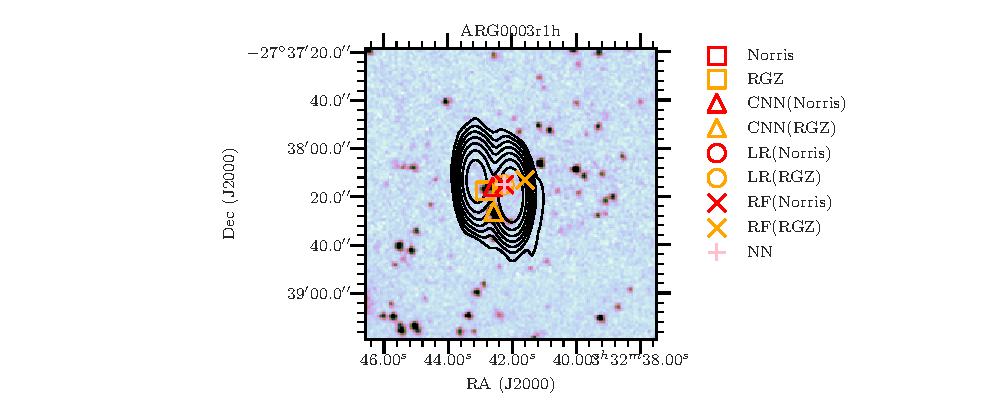
\includegraphics{atlas-images/examples_all/example_sorted_0_306.pdf}}
      % \subfloat[]{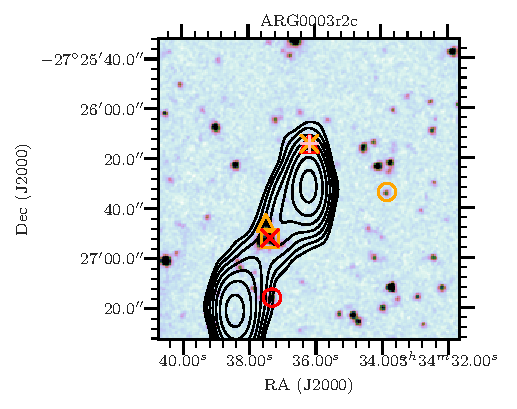
\includegraphics{atlas-images/examples_all/example_sorted_1_425.pdf}}

      \subfloat[]{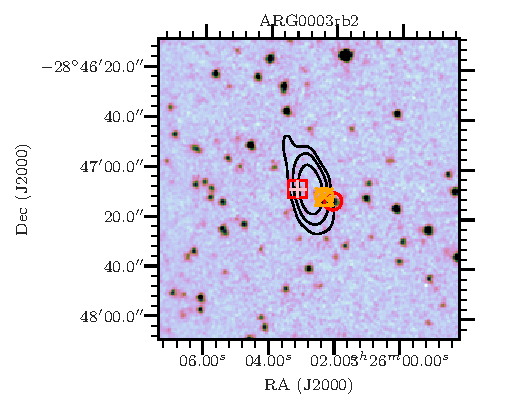
\includegraphics{atlas-images/examples_all/example_sorted_2_0.pdf}}%
      \subfloat[]{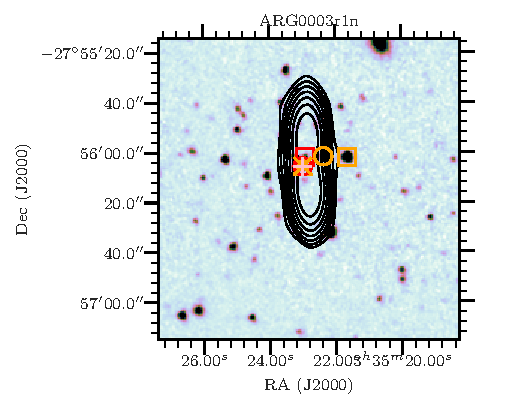
\includegraphics{atlas-images/examples_all/example_sorted_3_454.pdf}}

      \subfloat[]{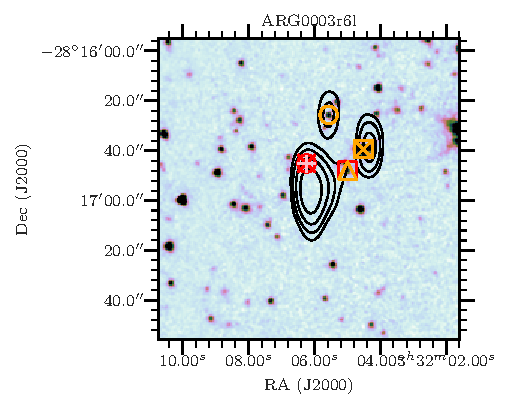
\includegraphics{atlas-images/examples_all/example_sorted_4_264.pdf}}%
      \subfloat[]{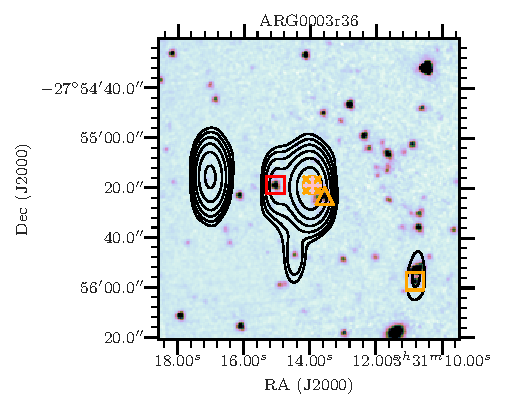
\includegraphics{atlas-images/examples_all/example_sorted_5_207.pdf}}
      \caption{\label{fig:examples} Examples of resolved sources with high disagreement between cross-identifiers. The contours show ATLAS radio data and start at $4\sigma$, increasing geometrically by a factor of 2. The background image is the \unit{3.6}{\micro\meter} SWIRE image. Binary classifier model/training set combinations are denoted $C(S)$ where $C$ is the binary classifier model and $S$ is the training set. `LR' is logistic regression, `CNN' is convolutional neural networks, and `RF' is random forests. `Norris' refers to the expert labels and `RGZ' refers to the Radio Galaxy Zoo labels. The cross-identification made by nearest-neighbours is shown by `NN'. The complete set of figures for 469 examples is available in the supplementary information.}
    \end{figure*}


  \section{2-Wasserstein begets Faraday moments}
  \label{sec:faraday-w2-to-faraday-moments}
    The 2-Wasserstein distance (\autoref{eq:w2}) gives the second Faraday moment (\autoref{eq:model-moment}) on a model FDF (\autoref{eq:true-fdf}). Let $\tilde F$ be the model FDF normalised as in \autoref{eq:normalised} and let $\tilde S$ be the normalised simple model FDF:
    \begin{align}
      \tilde F(\phi) &= \frac{A_0 \delta(\phi - \phi_0) + A_1 \delta(\phi - \phi_1)}{A_0 + A_1}\\
      \tilde S(\phi) &= \delta(\phi - \phi_w).
    \end{align}
    The set of couplings $\Gamma(\tilde F, \tilde S)$ is the set of all joint probability distributions $\gamma$ such that
    \begin{align}
      \int_{\phi_{\min}}^{\phi_{\max}} \gamma(\phi, \varphi)\ \mathrm{d}\phi &= \tilde S(\varphi),\\
      \int_{\phi_{\min}}^{\phi_{\max}} \gamma(\phi, \varphi)\ \mathrm{d}\varphi &= \tilde F(\phi).
    \end{align}
    The coupling that minimises the integral in \autoref{eq:w2} will be the optimal transport plan between $\tilde F$ and $\tilde S$. Since $\tilde F$ and $\tilde S$ are defined in terms of delta functions, the optimal transport problem reduces to a discrete optimal transport problem and the optimal transport plan is:
    \begin{equation}
      \gamma(\phi, \varphi) = \frac{A_0 \delta(\phi - \phi_0) + A_1 \delta(\phi - \phi_1)}{A_0 + A_1} \delta(\varphi - \phi_w).
    \end{equation}
    In other words, to move the probability mass of $\tilde S$ to $\tilde F$, a fraction $A_0/(A_0 + A_1)$ is moved from $\phi_w$ to $\phi_0$ and the complementary fraction $A_1/(A_0 + A_1)$ is moved from $\phi_w$ to $\phi_1$. Then:
    \begin{align}
      D_{W_2}\infdivx{\tilde F}{\tilde S}^2 &= \iint_{\phi_{\min}}^{\phi_{\max}} |\phi - \varphi|^2\ \mathrm{d}\gamma(\phi, \varphi)\\
        &= \frac{\iint_{\phi_{\min}}^{\phi_{\max}} (A_0 \delta(\phi - \phi_0) + A_1 \delta(\phi - \phi_1)) \delta(\varphi - \phi_w) (\phi - \varphi)^2\ \mathrm{d}\phi\ \mathrm{d}\varphi}{A_0 + A_1}\\
        &= \frac{\int_{\phi_{\min}}^{\phi_{\max}} (A_0 \delta(\phi - \phi_0) + A_1 \delta(\phi - \phi_1)) (\phi - \phi_w)^2\ \mathrm{d}\phi}{A_0 + A_1}\\
        &= \frac{A_0 (\phi_0 - \phi_w)^2 + A_1 (\phi_1 - \phi_w)^2}{A_0 + A_1}.
    \end{align}
    To obtain a Faraday complexity score (\autoref{eq:complexity-model}) we need to minimise this over $\phi_w$. Differentiate with respect to $\phi_w$ and set equal to zero to find
    \begin{equation}
      \phi_w = \frac{A_0 \phi_0 + A_1 \phi_1}{A_0 + A_1}.
    \end{equation}
    Substituting this back in, we find
    \begin{align}
      \varsigma_{W_2}(F)^2 &= \frac{A_0 (\phi_0 - \frac{A_0 \phi_0 + A_1 \phi_1}{A_0 + A_1})^2 + A_1 (\phi_1 - \frac{A_0 \phi_0 + A_1 \phi_1}{A_0 + A_1})^2}{A_0 + A_1}\\
        &= \frac{A_0 (A_1 (\phi_0 - \phi_1))^2 + A_1 (A_0 (\phi_1 - \phi_0))^2}{(A_0 + A_1)^3}\\
        &= \frac{A_0 A_1^2 (\phi_0 - \phi_1)^2 + A_0^2 A_1 (\phi_0 - \phi_1)^2}{(A_0 + A_1)^3}\\
        &= \frac{(A_0 A_1^2 + A_0^2 A_1) (\phi_0 - \phi_1)^2}{(A_0 + A_1)^3}\\
        &= \frac{A_0 A_1}{A_0 + A_1}(\phi_0 - \phi_1)^2
    \end{align}
    which is the Faraday moment.

  \section{Calculating W$_2$}
  \label{sec:faraday-pot}

    We used \texttt{Python Optimal Transport} \citep[\texttt{POT};][]{flamary17pot} to calculate W$_2$. \texttt{POT} implements a function \texttt{emd\_1d\_sorted} which solves the one-dimensional optimal transport problem for sorted coordinates. For coordinates $u = [u_1, \dots, u_d], v = [v_1, \dots, v_d]$ with weights $w = [w_1, \dots, w_d], s = [s_1, \dots, s_d]$, \texttt{POT} implements the following equation:
    \begin{equation}
      D_{\mathrm{W}_2} = \sum_{i = 1}^d |u_i - v_i|^2
    \end{equation}
    \todo{}

\section{Euclidean distance in the no-RMSF case}
\label{sec:faraday-euclidean-calculation}

  In this section we calculate the minimumised Euclidean distance evaluated on a model FDF (\autoref{eq:true-fdf}). Let $\tilde F$ be the model FDF normalised as in \autoref{eq:normalised} and let $\tilde S$ be the normalised simple model FDF:
  \begin{align}
    \tilde F(\phi) &= \frac{A_0 \delta(\phi - \phi_0) + A_1 \delta(\phi - \phi_1)}{A_0 + A_1}\\
    \tilde S(\phi; \phi_e) &= \delta(\phi - \phi_e).
  \end{align}

  The Euclidean distance between $\tilde F$ and $\tilde S$ is then
  \begin{align}
    D_E\infdivx{\tilde F(\phi)}{\tilde S(\phi; \phi_e)}^2 &= \int_{\phi_{\min}}^{\phi_{\max}} \left|\frac{A_0 \delta(\phi - \phi_0) + A_1 \delta(\phi - \phi_1)}{(A_0 + A_1)^2} - \delta(\phi - \phi_e) \right|^2\ \mathrm{d}\phi\\
      &= \frac{1}{(A_0 + A_1)^2} \int_{\phi_{\min}}^{\phi_{\max}} \left|A_0 \delta(\phi - \phi_0) + A_1 \delta(\phi - \phi_1) - (A_0 + A_1) \delta(\phi - \phi_e) \right|^2\ \mathrm{d}\phi\\
      &= \frac{1}{(A_0 + A_1)^2} \int_{\phi_{\min}}^{\phi_{\max}} \begin{cases}
        A_1^2 \left|\delta(\phi - \phi_1) - \delta(\phi - \phi_0) \right|^2, & \phi_e = \phi_0\\
        A_0^2 \left|\delta(\phi - \phi_0) - \delta(\phi - \phi_1) \right|^2, & \phi_e = \phi_1\\
        \left|A_0 \delta(\phi - \phi_0) + A_1 \delta(\phi - \phi_1) - (A_0 + A_1) \delta(\phi - \phi_e) \right|^2, & \mathrm{else}\\
      \end{cases}\ \mathrm{d}\phi\\
      &= \begin{cases}
        \begin{cases}
          \frac{2 A_1^2}{(A_0 + A_1)^2}, & \phi_e = \phi_0\\
          \frac{2 A_0^2}{(A_0 + A_1)^2}, & \phi_e = \phi_1\\
          \frac{A_0^2 + A_1^2 + 1}{(A_0 + A_1)^2}, & \mathrm{else}\\
        \end{cases} & \phi_0 \neq \phi_1\\
        \begin{cases}
          0, & \phi_e = \phi_0\\
          2, & \phi_e \neq \phi_0\\
        \end{cases} & \phi_0 = \phi_1\\
      \end{cases}\ \mathrm{d}\phi.\\
  \end{align}
  Assuming $\phi_0 \neq \phi_1$, then the minimised Euclidean distance is
  \begin{align}
      D_E(F) &= \min_{\phi_e \in \mathbb{R}} D_E\infdivx{F(\phi)}{F_{\mathrm{simple}}(\phi; \phi_e)}\\
          &= \sqrt{2} \frac{\min(A_0, A_1)}{A_0 + A_1}.
  \end{align}
  If $\phi_0 = \phi_1$, then the minimised Euclidean distance is 0.

\section{Thresholds for precision and recall}
\label{sec:faraday-thresholds-pr}

  \todo{Add a page documenting thresholds optimised for both precision and recall. Motivate these: Which scenarios would we care about precision? Recall? (Hint: depends whether you want complex or simple sources!)}

\section{Minimisation over simple FDFs}
\label{sec:faraday-minimisation}

  As part of our method, we need to minimise a divergence function $D_f$ over the manifold of simple FDFs $\hat F_{\mathrm{simple}}$:
  \begin{equation}
      \varsigma_f(\hat F) = \min_{\phi_w \in \mathbb{R}} D_f\infdivx{\hat F(\phi)}{\hat F_{\mathrm{simple}}(\phi; \phi_s)}.
  \end{equation}
  To do this, we perform a two-step approach. This two-step approach allows us to find a smooth (i.e. not discretised) minimum without encountering local minima due to the non-convexity of the optimisation target. First, we generate 1~000 noise-free simple FDFs following \autoref{sec:simulated-fdfs} using the same frequencies as those used to observe $\hat F$, with $\sigma = 0$ and $\phi_0 \in \{\phi_{\min}, \phi_{\min} + \delta\phi, \dots, \phi_{\max}\}$. This is a discrete representation of the simple manifold. We then evaluate $D_f$ between our observed FDF $\hat F$ and these simple spectra and identify the $\phi_0$ that gives us the smallest value of $D_f\infdivx{\hat F(\phi)}{\hat F_{\mathrm{simple}}(\phi; \phi_0)}$. Call this $\phi_0^{(1)}$. This gives us an initial guess at the minimising value of $\phi_s$ in \autoref{eq:complexity-model}. Second, we use \texttt{scipy.optimize.fmin\textunderscore{}bfgs} to minimise $D_f\infdivx{\hat F(\phi)}{\hat F_{\mathrm{simple}}(\phi; \phi_s)}$ over $\phi_s$ using $\phi_0^{(1)}$ as an initial value, producing a new minimiser $\phi_0^{(2)}$.

\section{Hyperparameters for LR and XGB}
\label{sec:faraday-hyperparameters}

  \begin{table}
    \caption{\label{tab:faraday-hyperparameters-xgb} XGB hyperparameters for the Livingston dataset.}
    \begin{tabular}{ll}
      \hline\hline
      Parameter & Value\\\hline
      colsample\textunderscore{}bytree & 0.896\\
      gamma & 0.606\\
      learning\textunderscore{}rate & 0.1\\
      max\textunderscore{}depth & 5\\
      min\textunderscore{}child\textunderscore{}weight & 1\\
      scale\textunderscore{}pos\textunderscore{}weight & 1\\
      subsample & 0.690\\
      n\textunderscore{}estimators & 95\\
      reg\textunderscore{}alpha & 2.677\\
      reg\textunderscore{}lambda & 7.344\\
      \hline\hline
    \end{tabular}
  \end{table}

  \begin{table}
    \caption{\label{tab:faraday-hyperparameters-lr} LR hyperparameters for the Livingston dataset.}
    \begin{tabular}{ll}
      \hline\hline
      Parameter & Value\\\hline
      penalty & L2\\
      C & 0.464\\
      \hline\hline
    \end{tabular}
  \end{table}

  \begin{table}
    \caption{\label{tab:faraday-hyperparameters-xgb-askap12} XGB hyperparameters for the ASKAP-12 dataset.}
    \begin{tabular}{ll}
      \hline\hline
      Parameter & Value\\\hline
      colsample\textunderscore{}bytree & 0.865\\
      gamma & 0.256\\
      learning\textunderscore{}rate & 0.1\\
      max\textunderscore{}depth & 6\\
      min\textunderscore{}child\textunderscore{}weight & 1\\
      scale\textunderscore{}pos\textunderscore{}weight & 1\\
      subsample & 0.819\\
      n\textunderscore{}estimators & 108\\
      reg\textunderscore{}alpha & 0.049\\
      reg\textunderscore{}lambda & 0.454\\
      \hline\hline
    \end{tabular}
  \end{table}

  \begin{table}
    \caption{\label{tab:faraday-hyperparameters-lr-askap12} LR hyperparameters for the ASKAP-12 dataset.}
    \begin{tabular}{ll}
      \hline\hline
      Parameter & Value\\\hline
      penalty & L2\\
      C & 0.464\\
      \hline\hline
    \end{tabular}
  \end{table}
